\documentclass[tikz,border=5pt]{standalone}
\usepackage{tikz}
\usetikzlibrary{calc,angles,quotes,arrows.meta}

\begin{document}
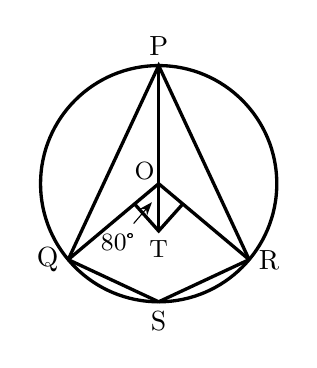
\begin{tikzpicture}

  % Radius
  \def\r{1.5}
  
  % Points on circle
  \coordinate (O) at (0, 0);
  \coordinate (P) at (90:\r);
  \coordinate (Q) at (220:\r);
  \coordinate (R) at (320:\r);
  \coordinate (S) at (-90:\r);
  
  % Point T on line PS between O and S
  \coordinate (T) at (0,-0.60);
  
  % Draw circle
  \draw[very thick] (0,0) circle (\r);
  
  % Draw lines
  \draw[very thick] (Q) -- (P) -- (R);
  \draw[very thick] (P) -- (T);
  \draw[very thick] (O) -- (Q);
  \draw[very thick] (O) -- (R);
  \draw[very thick] (S) -- (Q);
  \draw[very thick] (S) -- (R);
  
  % Angle marker at O (80°) - right angle style with corner at T
  \coordinate (A1) at ($(O)+(220:0.4)$);
  \coordinate (A2) at ($(O)+(320:0.4)$);
  \coordinate (A3) at (T);
  \draw[very thick] (A1) -- (A3) -- (A2);
  
  % Point labels
  \node[above] at (P) {P};
  \node[left] at (Q) {Q};
  \node[right] at (R) {R};
  \node[below] at (S) {S};
  \node[above left=-2pt, font=\small] at (O) {O};
  \node[below, font=\small] at (T) {T};
  
  % 80° angle label with arrow pointing to angle QOR
  \node[font=\small] at ($(O)+(235:0.9)$) (anglelabel) {80°};
  \draw[-{Stealth}, thin] (anglelabel) -- ($(O)+(250:0.25)$);
  
\end{tikzpicture}
\end{document}